%!TEX root = ../main.tex
\section{Results}

\subsection{Simulated Results}

The plane-based registration is applied to the simulated dataset with noisy pose and range measurements (cf. Figure~\ref{fig:simulatedDatasets}) without further processing.
Assuming this represents a coarsely pre-registered 3D point cloud, the distances to the ground truth were evaluated before and after the plane-based registration. 
Figure~\ref{fig:simulatedEvaluation} shows the different point-to-point distances. 

\begin{figure*}
 	\centering
 	\begin{minipage}[c]{0.495\textwidth}
 		\centering
		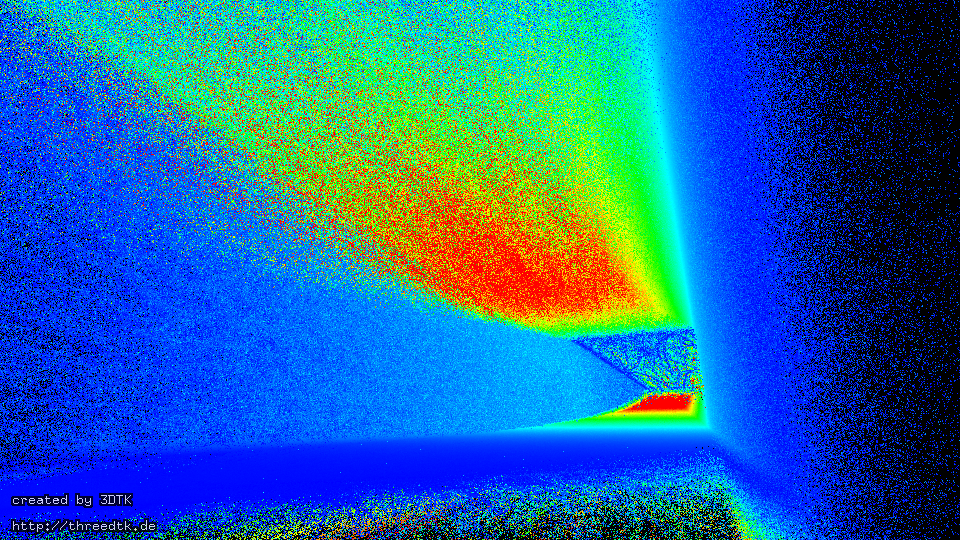
\includegraphics[width=\textwidth]{./images/uncorr_bottom_pose}\\
		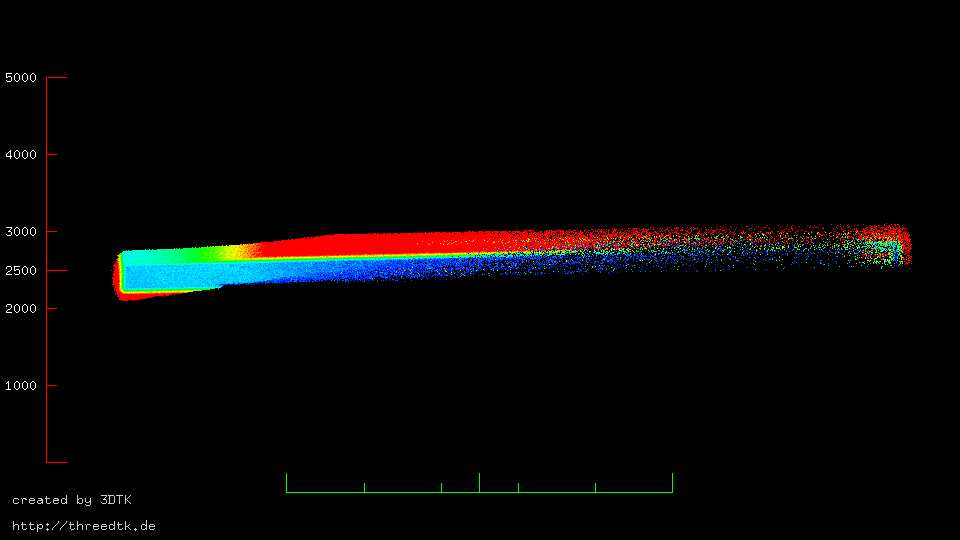
\includegraphics[width=\textwidth]{./images/uncorr_side_view}\\
  		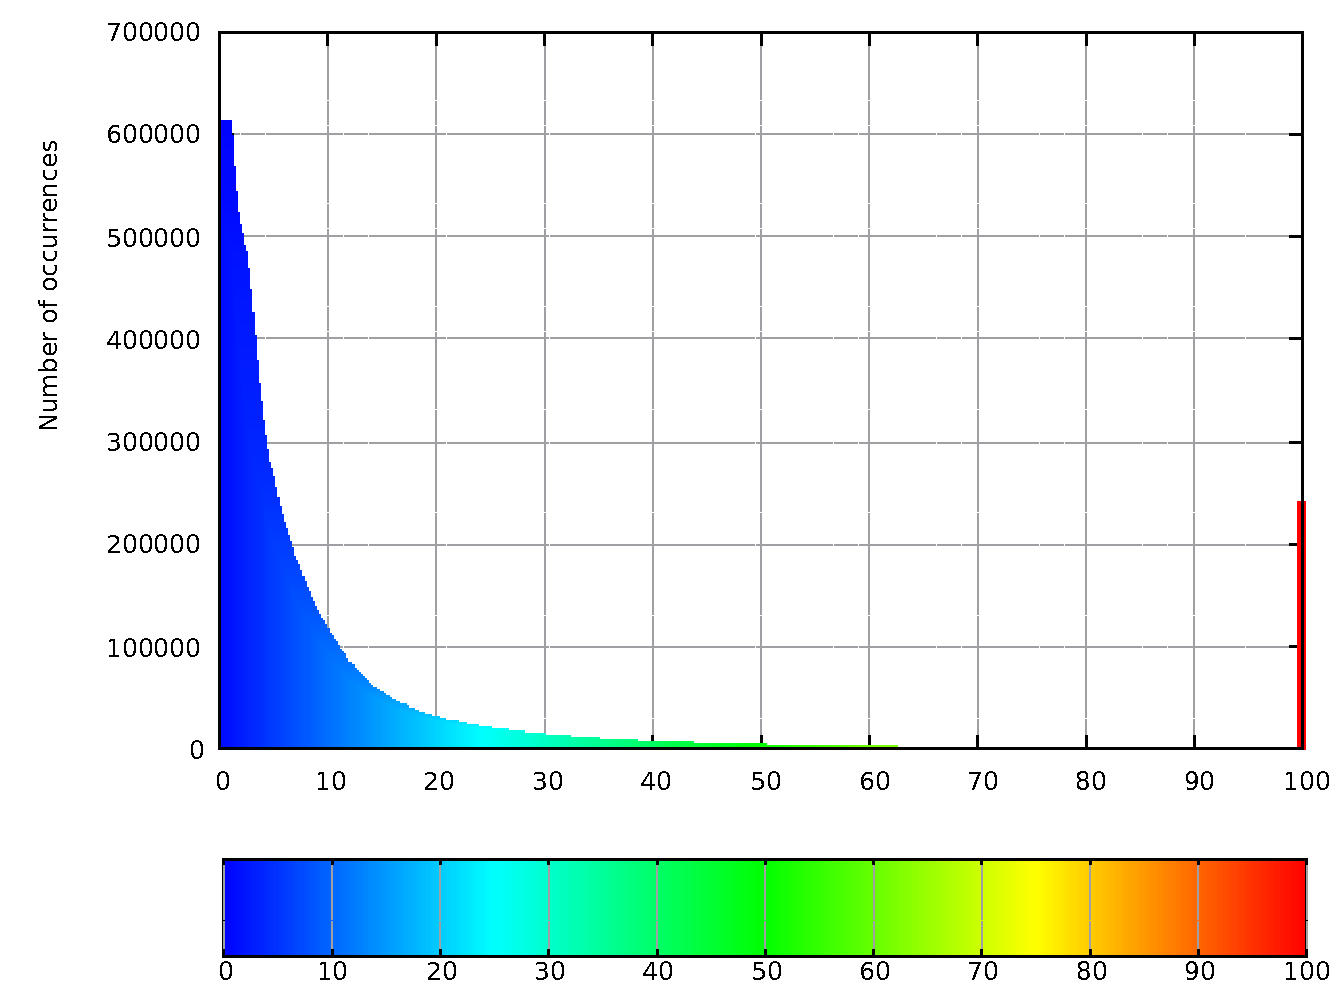
\includegraphics[width=\textwidth]{./images/uncorr_hist}
  	\end{minipage}\hfill
  	\begin{minipage}[c]{0.495\textwidth}
  		\centering
		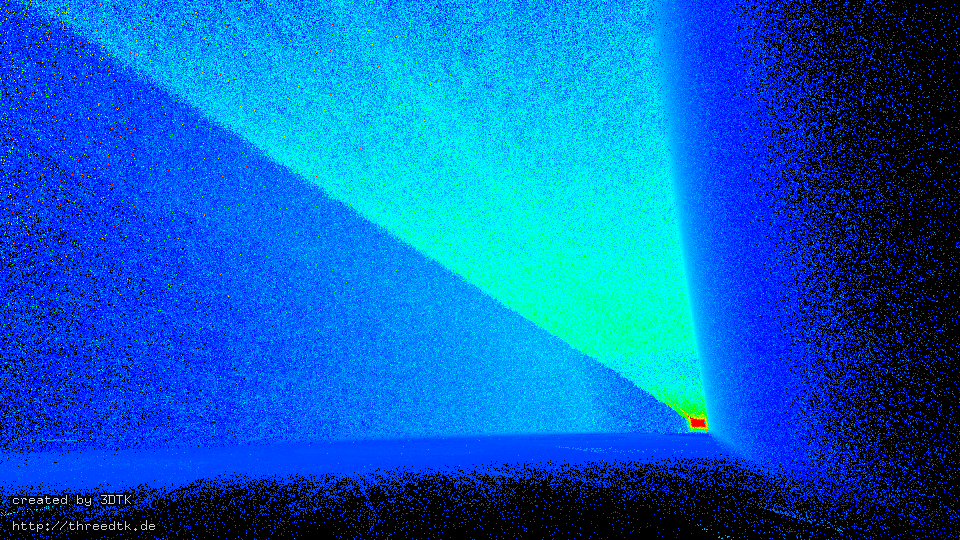
\includegraphics[width=\textwidth]{./images/corr_bottom_pose}\\
		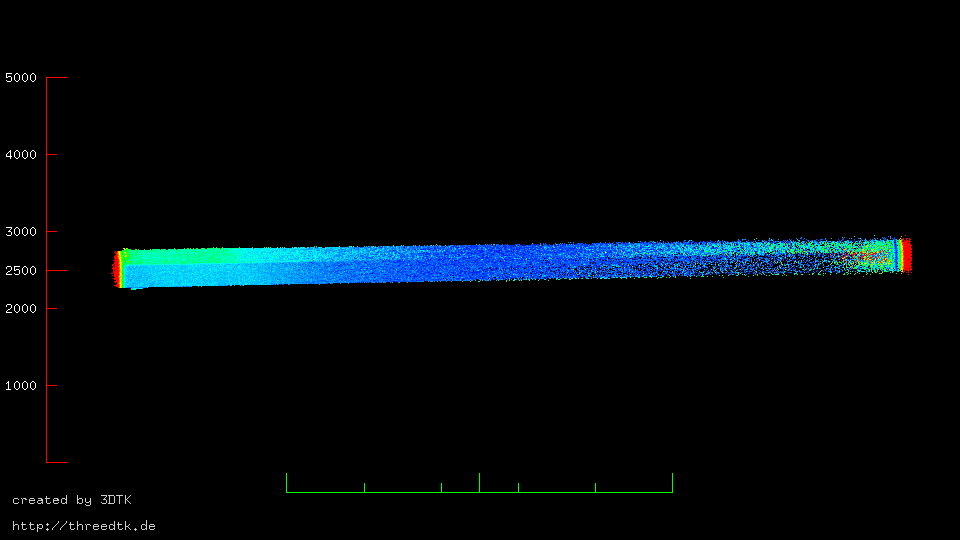
\includegraphics[width=\textwidth]{./images/corr_side_view}\\
  		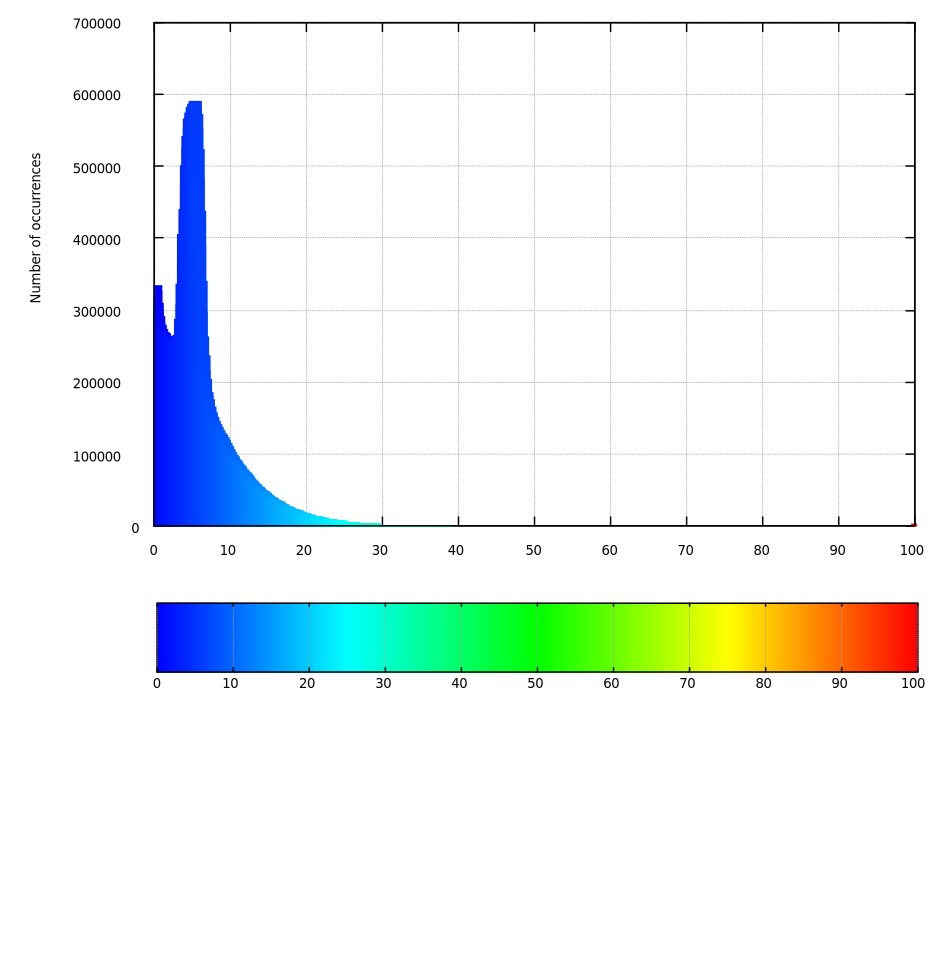
\includegraphics[width=\textwidth]{./images/corr_hist}
  	\end{minipage} 	
 	\caption{Evaluation of point distances before (left) and after (right) the plane-based registration on a simulated dataset. Lateral images always have the same orientation. A maximal distance of \SI{30}{m} is set, such that all points that display a higher distance value are excluded from the analysis. Both point-clouds were reduced before evaluating point-to-point distances to the ground-truth. Further, the color-space maps all values with a distance greater than \SI{1}{m} to the same color. The top two columns show a heat map of distances, while the bottom shows the corresponding histogram. The color mapping is equivalent in both. An animation of the matching process is given at \url{https://youtu.be/7igQdEeCsYk}.} 
 	\label{fig:simulatedEvaluation}
\end{figure*} 

Before the registration, the corridor is only represented acceptably in the front part. 
The further into the corridor, i.e., the longer the robot accumulates errors, the more imprecise the data becomes. 
Finally, we see that many points exceed the threshold of \SI{1}{\meter} and thus being mapped to the same color value.
After registration, we see that, qualitatively, the ideal corridor was nearly restored from the noisy data. 
In particular a very large portion of points (90\%) have distances of less than \SI{35.9}{\centi\meter}.
Table~\ref{tab:percentiles} shows the comparison of further percentiles of both datasets. 

\begin{table}
	\centering
	\begin{tabular}{@{}lccc@{}}\hline
		& P90 & P95 & P98 \\ \hline\hline
		Uncorrected & \SI{372.1}{\centi\meter} &  \SI{553.4}{\centi\meter} &  \SI{827.9}{\centi\meter} \\%& \SI{9.7}{\centi\meter}\\
		Corrected & \SI{35.9}{\centi\meter} &  \SI{64.1}{\centi\meter} &  \SI{122.8}{\centi\meter} \\\hline%& \SI{6.3}{\centi\meter}\\ \hline
	\end{tabular}
	\caption{Comparison of point-distances in the uncorrected and corrected simulated dataset.}
	\label{tab:percentiles}
\end{table}

Further, the square and straight shape of the corridor is restored well, and especially the large amount of points with an errors of greater than \SI{1}{m} is removed. 
Any such errors tend to occur at the back and the front of the corridor where the measured range is the largest hence has the largest contribution of the range error. 

\subsection{Floating Sphere Results}

Figure~\ref{fig:cylon-corrected} shows the results obtained before and after employing the plane based registration on the dataset acquired by the floating sphere.
The pre-registration is obtained by determining the orientation of the sphere via Madgwick filtered~\cite{madgwick2010efficient} IMU measurements.
To increase the number of possible point-to-plane correspondences we combine twenty temporally successive scans into one meta-scan, which is then globally registered. 
We always use the scan at the median index as a reference coordinate system.
This does not only speed up convergence due to the proportional effect on the error function but also decreases the risk of transforming a single line scan incorrectly.
Transformations like these happen in particular for a small collection of points as outliers have more influence.

\begin{figure*}
	\centering
	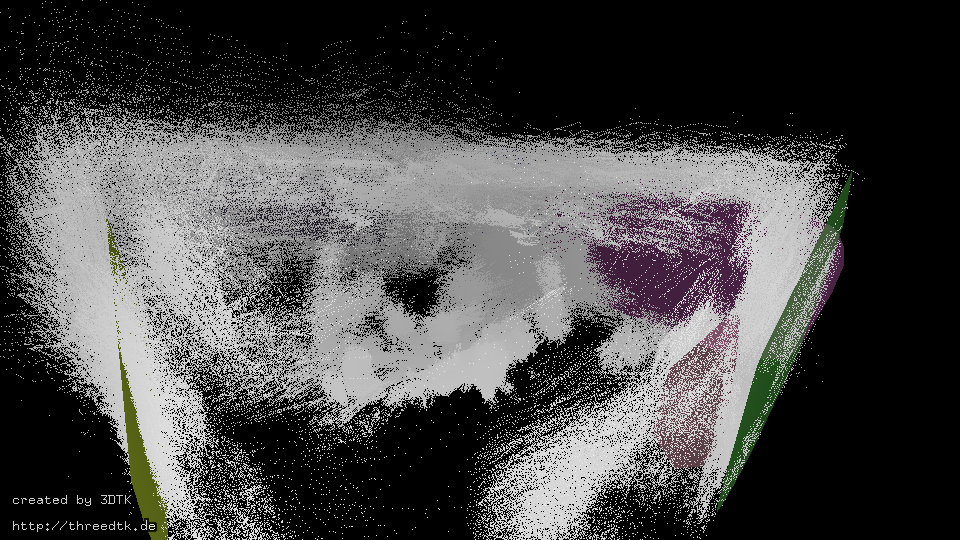
\includegraphics[width=0.495\textwidth]{./images/cylon_uncorr_corner}\hfill
	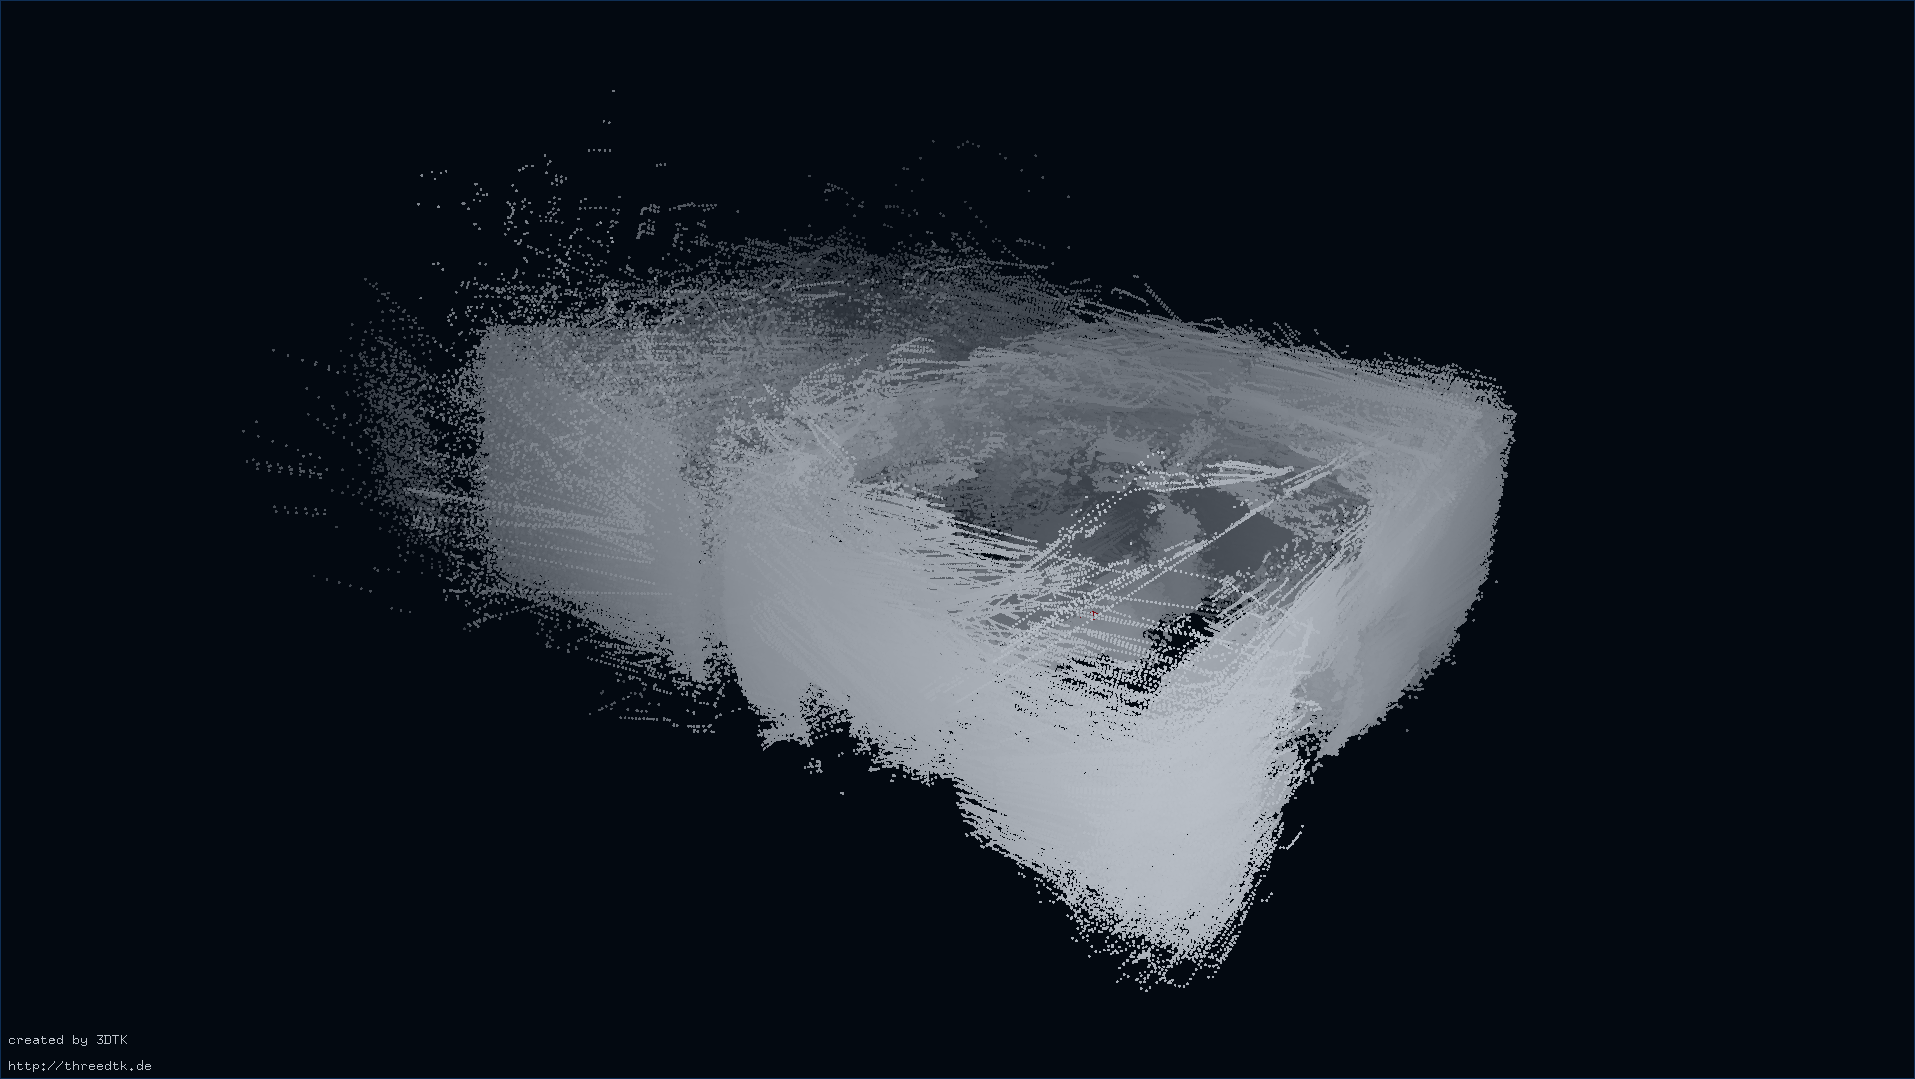
\includegraphics[width=0.495\textwidth]{./images/cylon_corr_corner}\\
	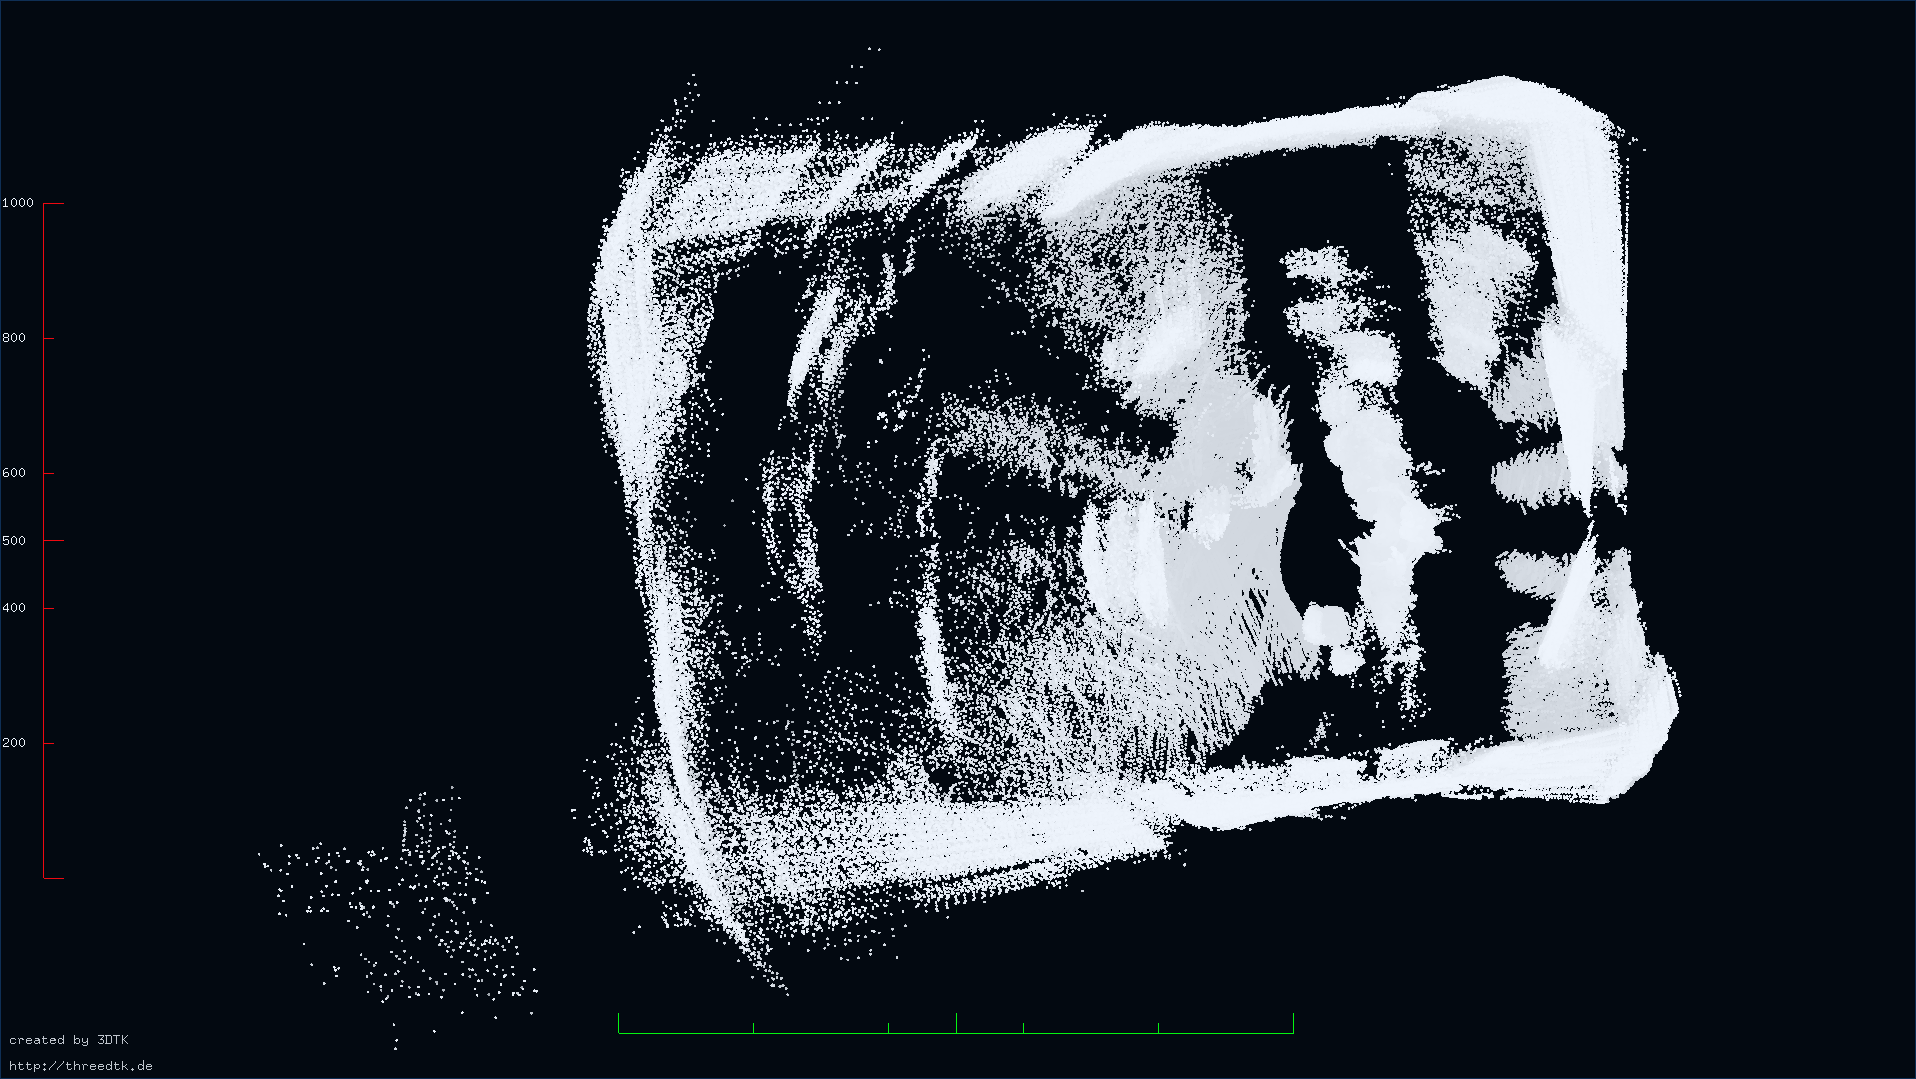
\includegraphics[width=0.495\textwidth]{./images/cylon_uncorr_top}\hfill
	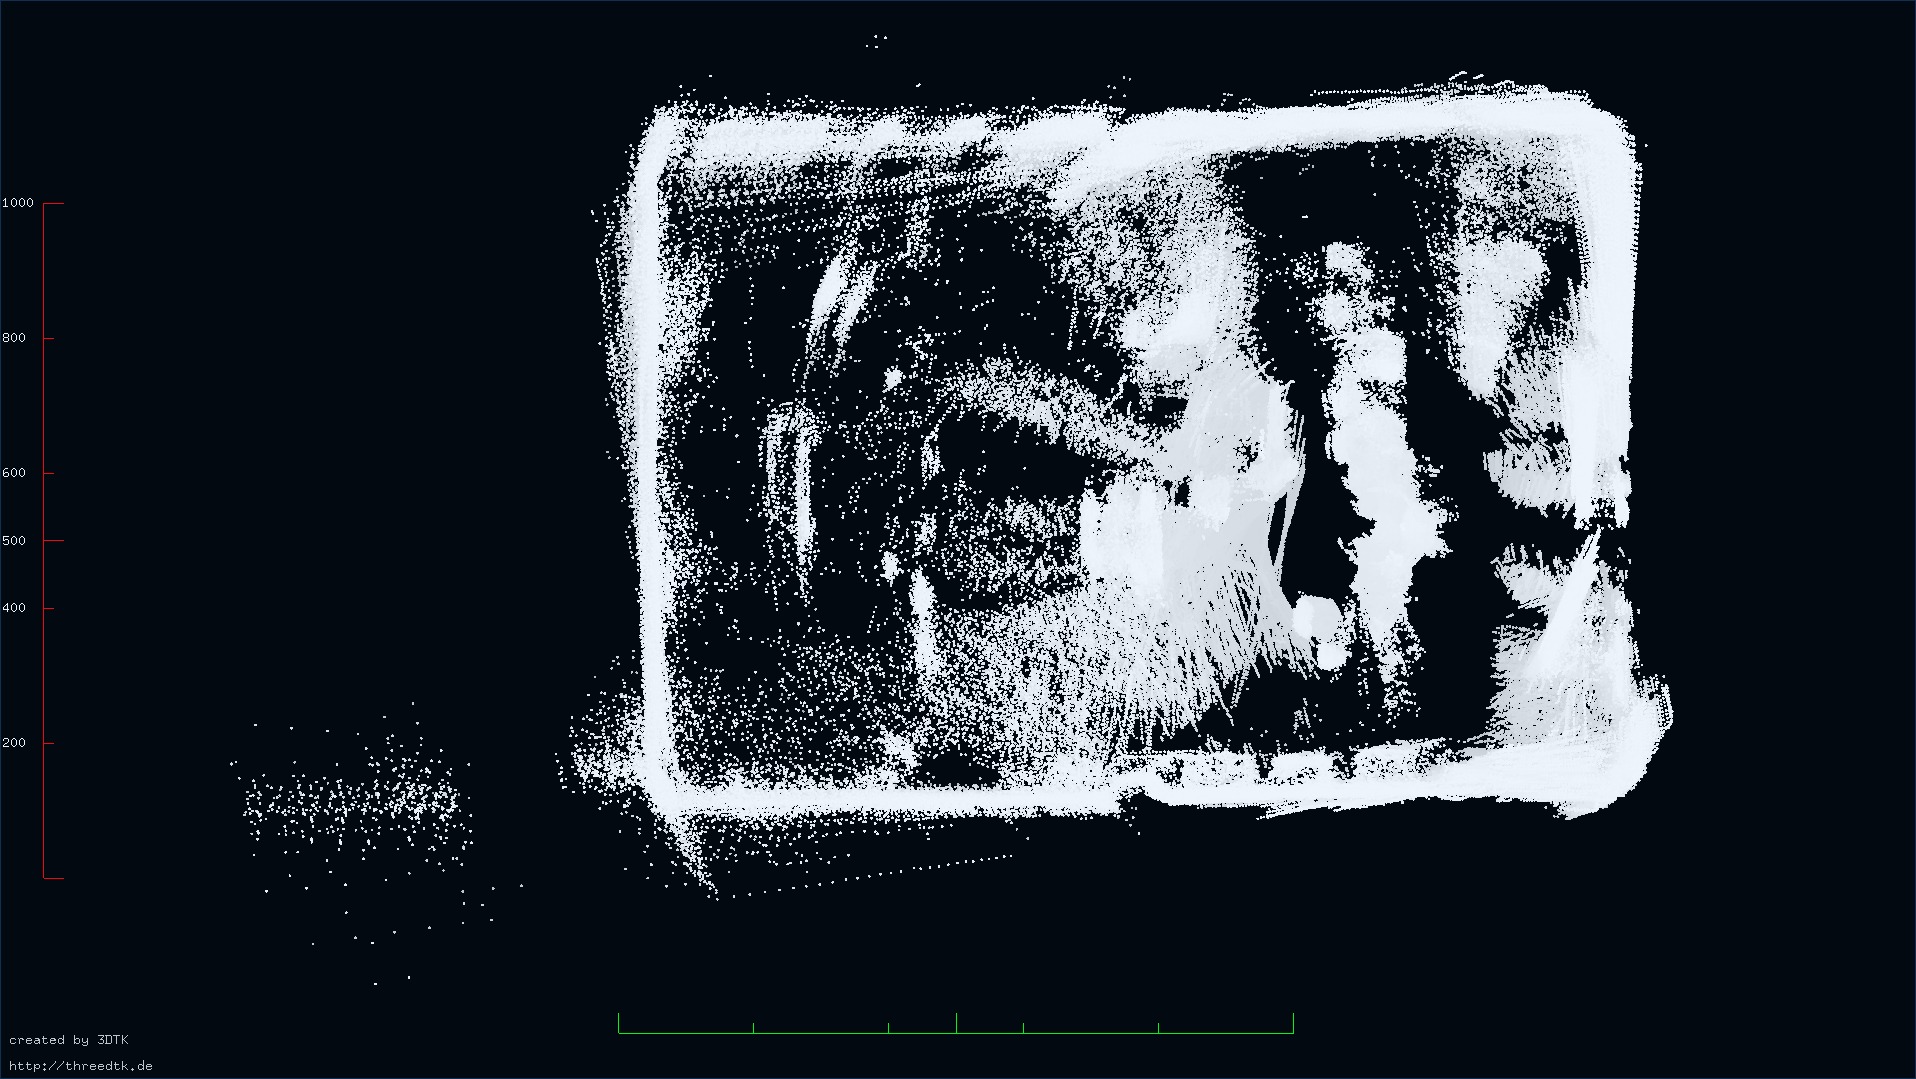
\includegraphics[width=0.495\textwidth]{./images/cylon_corr_top}
	\caption{The point cloud acquired by the floating sphere before (left) and after (right) applying the plane based registration. View from the interior (top) and a birds-eye view (bottom). Parameters used for optimization: $\epsilon_H = 50$, $\epsilon_P = 200$, $\epsilon_\alpha = \frac{\pi}{4}$, $K = 20$ for AKNN, $d_{growth} = 50$, $N_{c_min} = 200$, $\alpha_0 = [0.01, 0.01, 0.01, 0, 0, 0]^\tau$, $i = 8$, $k = 100$. An animation of the registration process is given at \url{https://youtu.be/Qa2Qi8z0KEk} .}
	\label{fig:cylon-corrected}
\end{figure*}
After the registration, the walls of the room are significantly more prominent in the point cloud. 
In particular, the noise in the top left corner of the top view (cf. figure~\ref{fig:cylon-corrected}) has been visibly reduced.
Further, the deviation of points around the walls is notably smaller as the points are moved on the plane.

\subsection{Rolling Sphere Results}

Figure~\ref{fig:jasperhome} shows the results obtained before and after employing the presented algorithm on the dataset, acquired by the prototype in figure~\ref{fig:prototype}.
We again combine twenty temporally successive scans into one meta-scan, using the scan at the median index as a reference coordinate system, which is then globally registered.
We used the first seven of these meta-scans, corresponding to the first full rotation of the spher, to extract global planes.
All subsequent meta-scans are then matched against the initial global plane model.
We use both optimizations from section \ref{ssec:furtheropts}, introducing a global up/down lock for gradient descent and applying sequential iteration to eliminate accumulating pose error.


\begin{figure*}
        \centering
        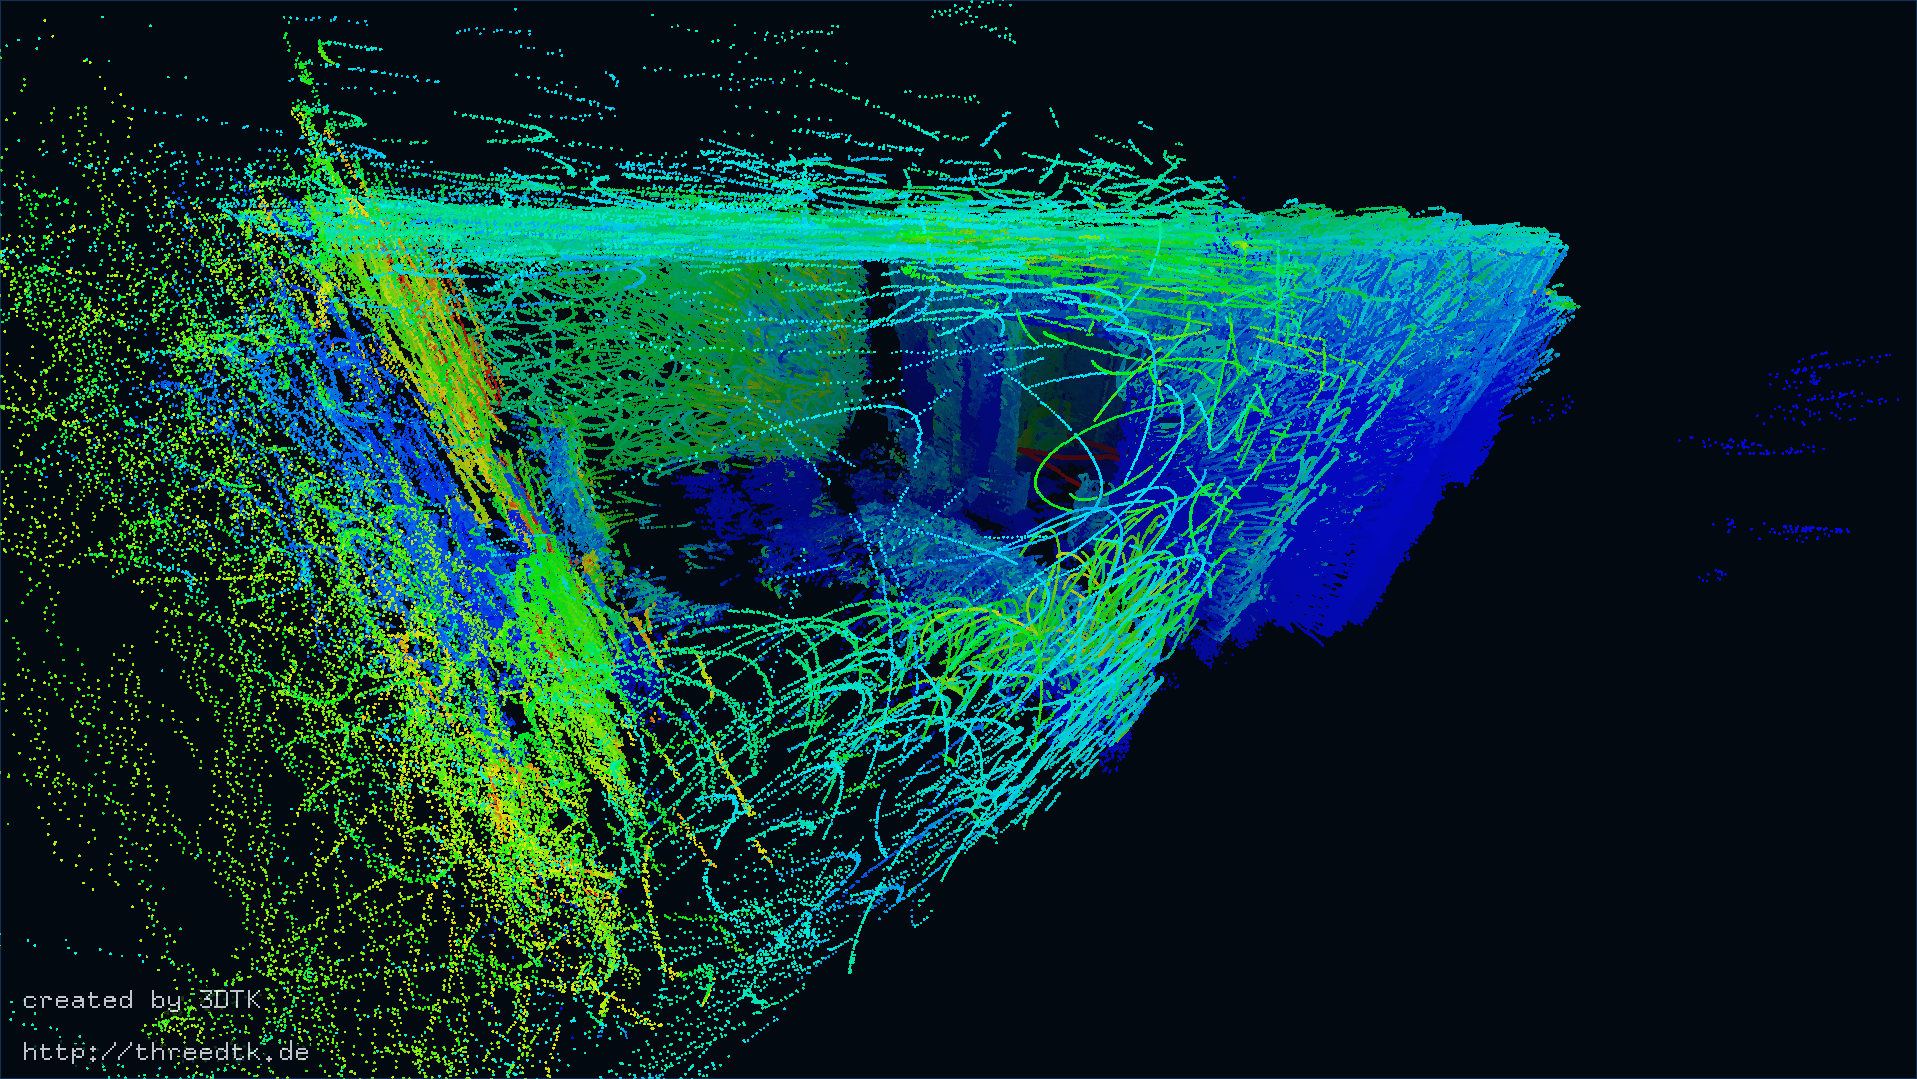
\includegraphics[width=0.495\textwidth]{./images/jasper_uncorr_corner}\hfill
        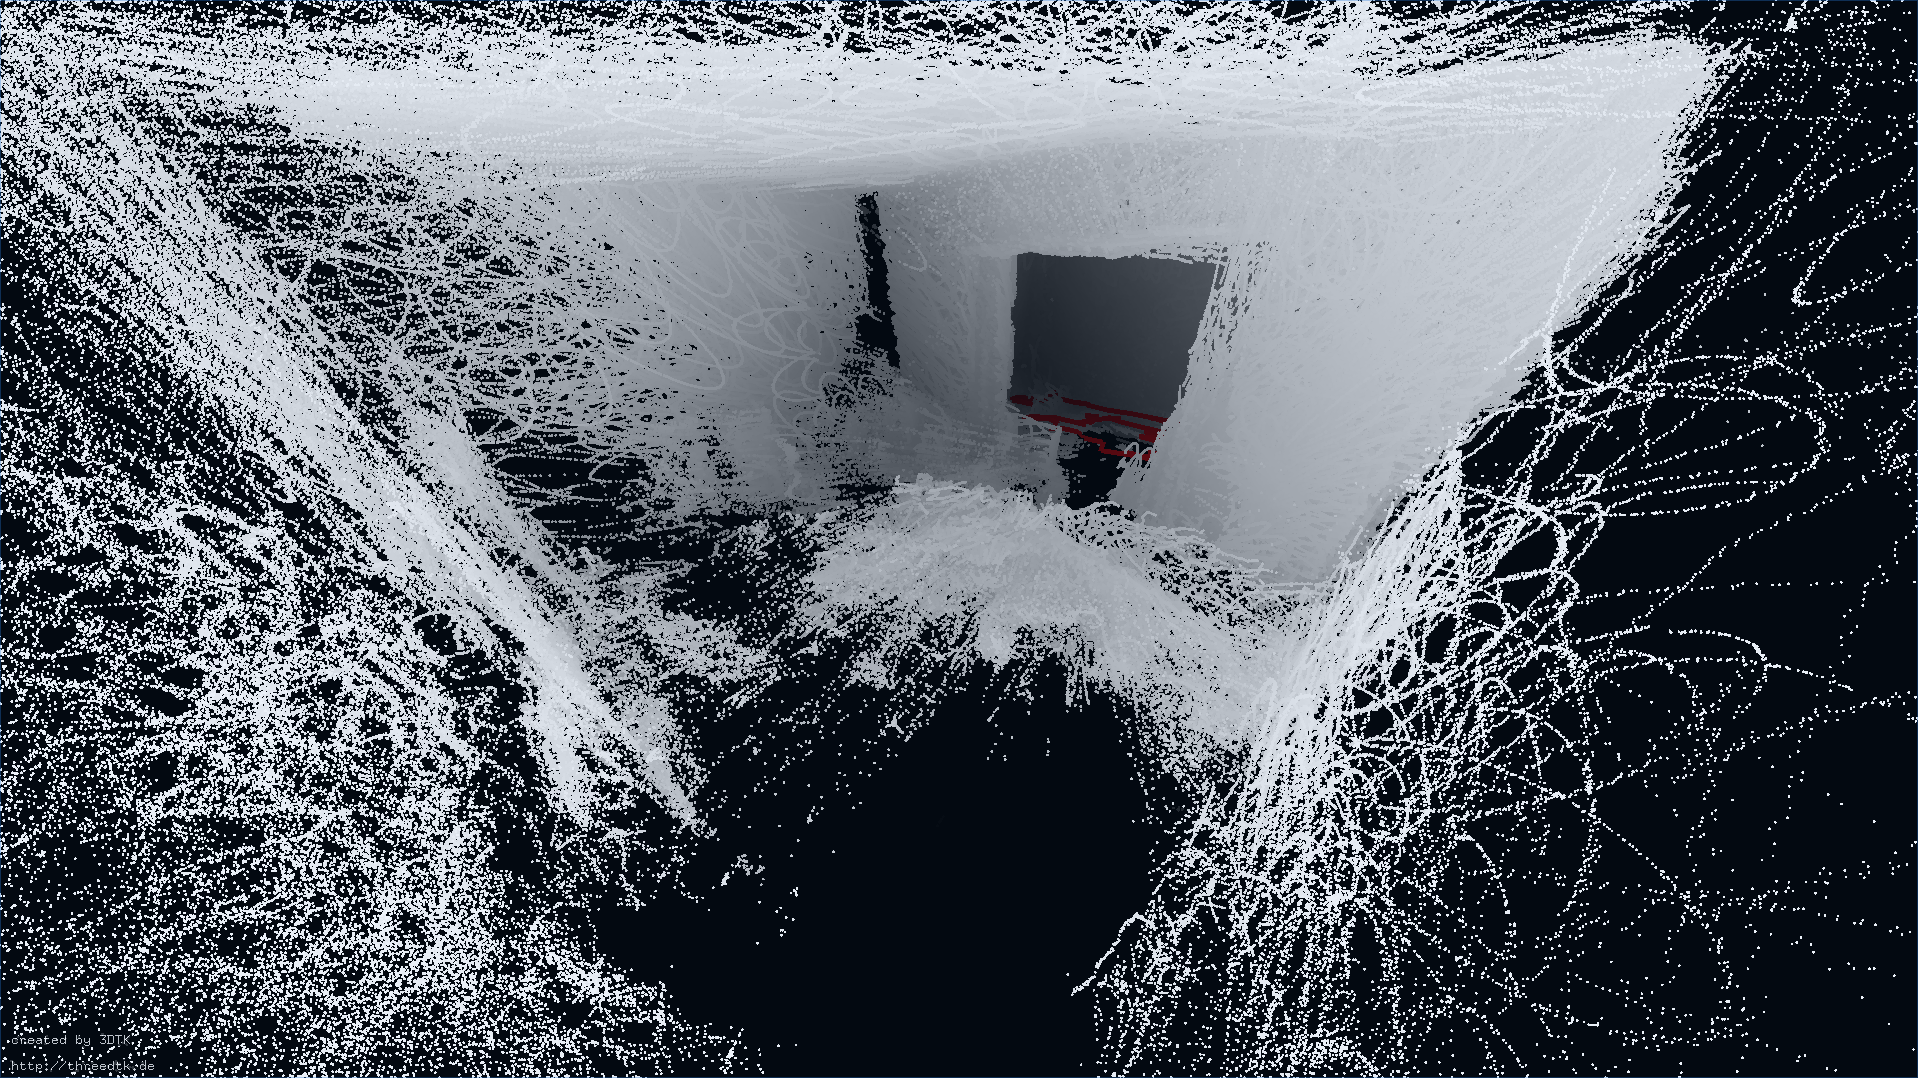
\includegraphics[width=0.495\textwidth]{./images/jasper_corr_corner}\\
	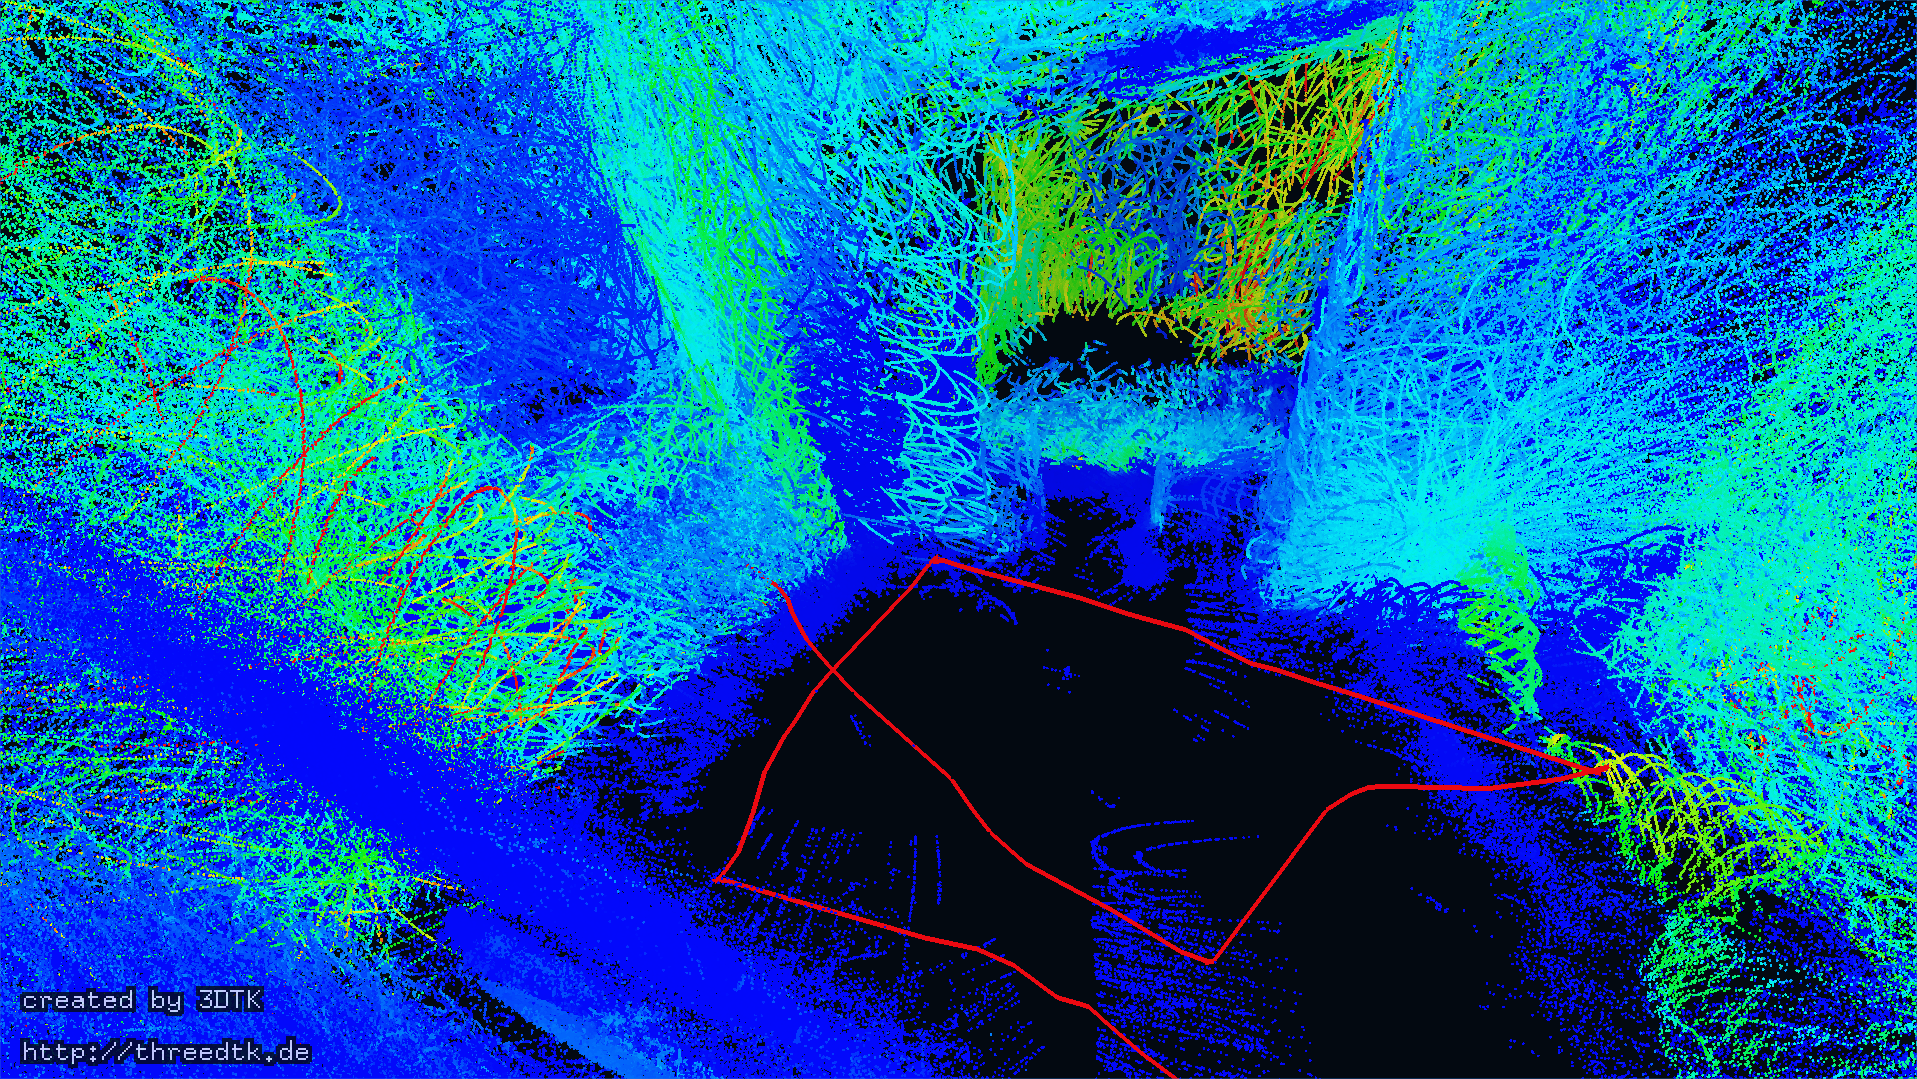
\includegraphics[width=0.495\textwidth]{./images/jasper_uncorr_color}\hfill
	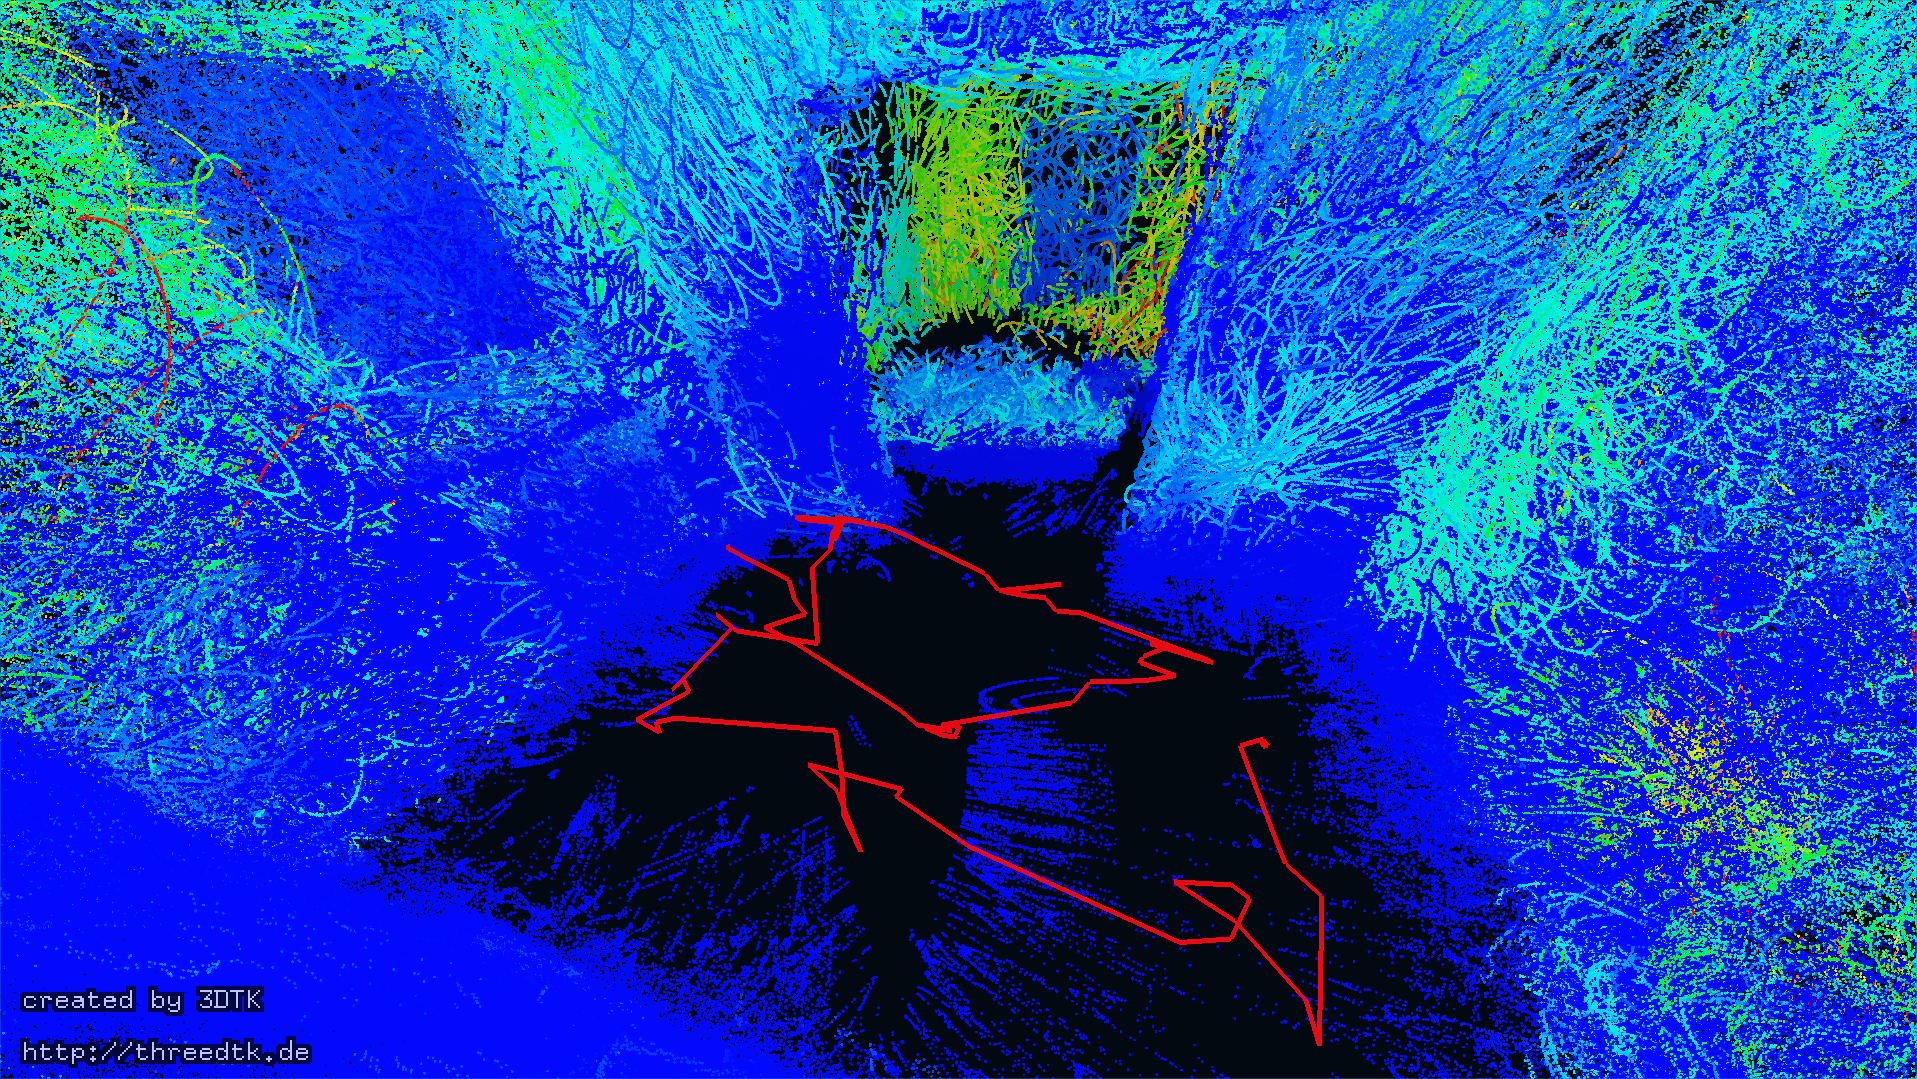
\includegraphics[width=0.495\textwidth]{./images/jasper_corr_color}\\
        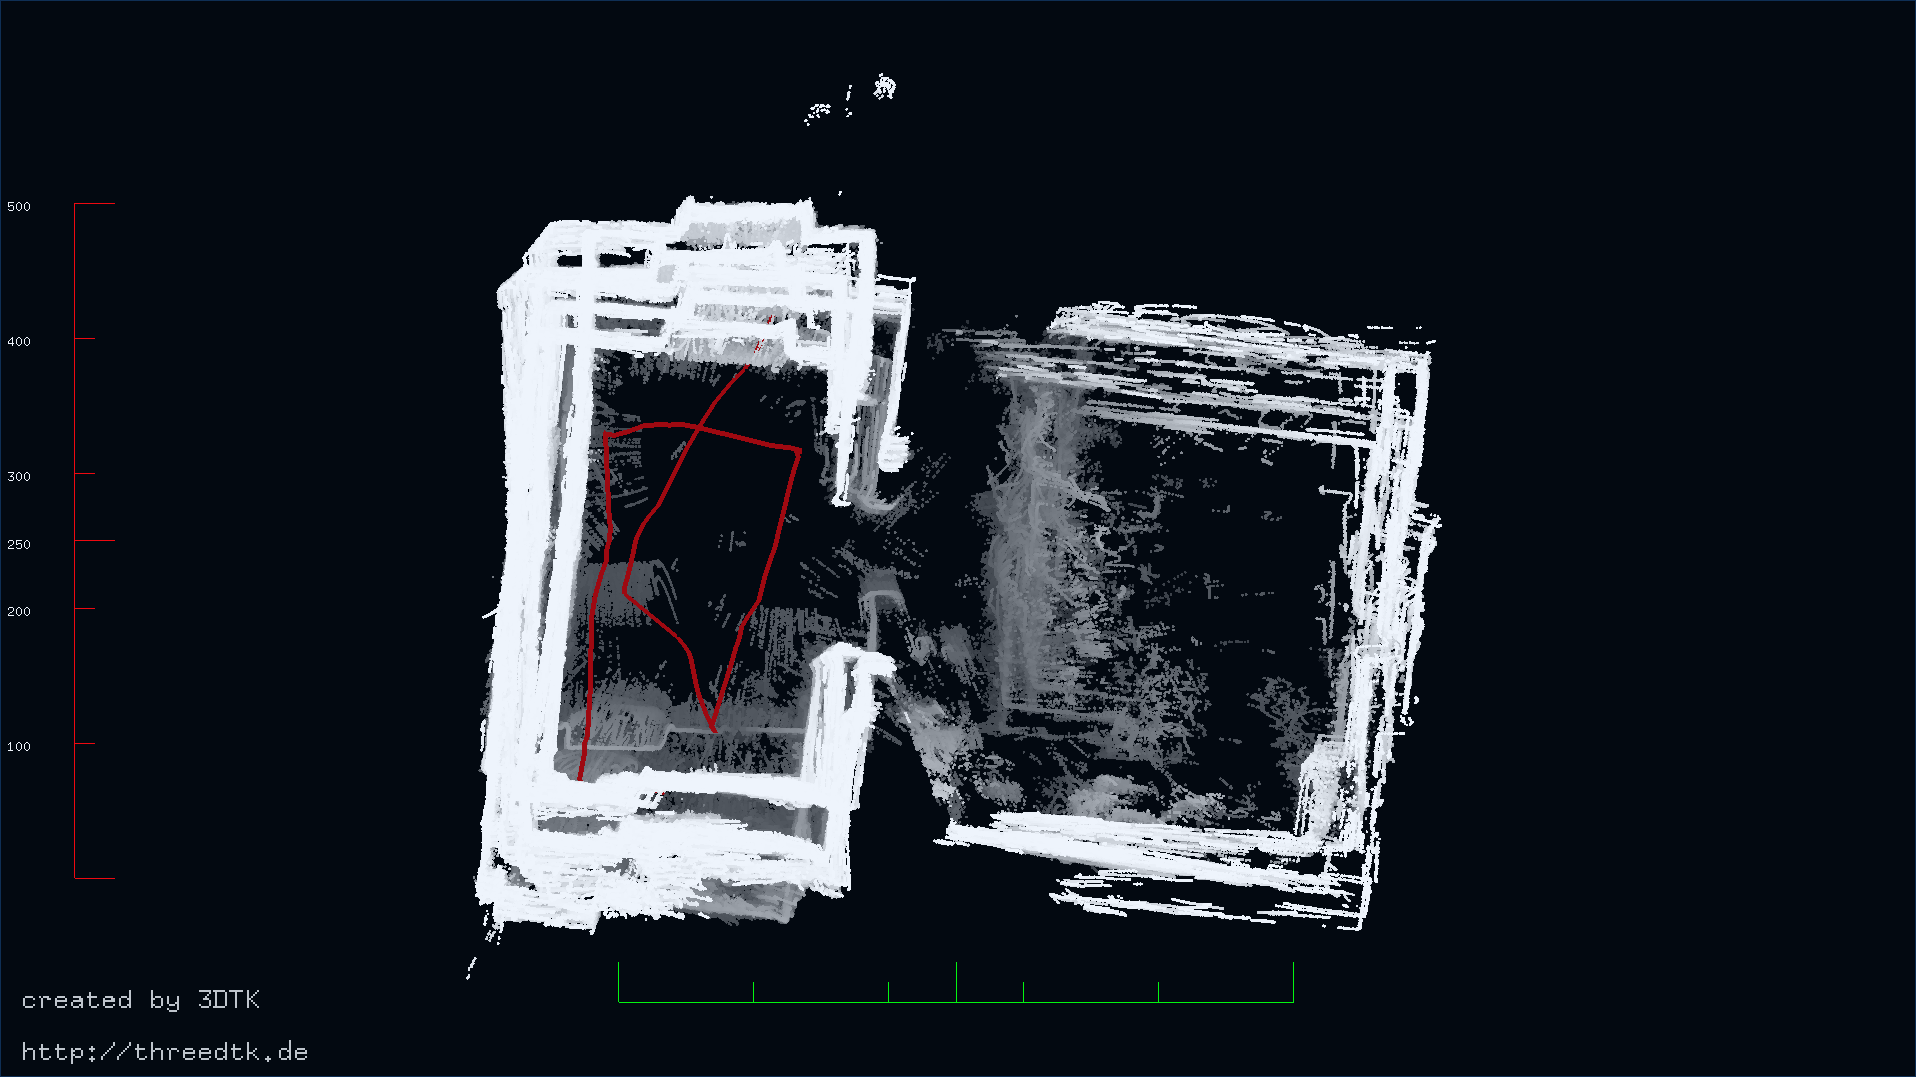
\includegraphics[width=0.495\textwidth]{./images/jasper_uncorr_top}\hfill
        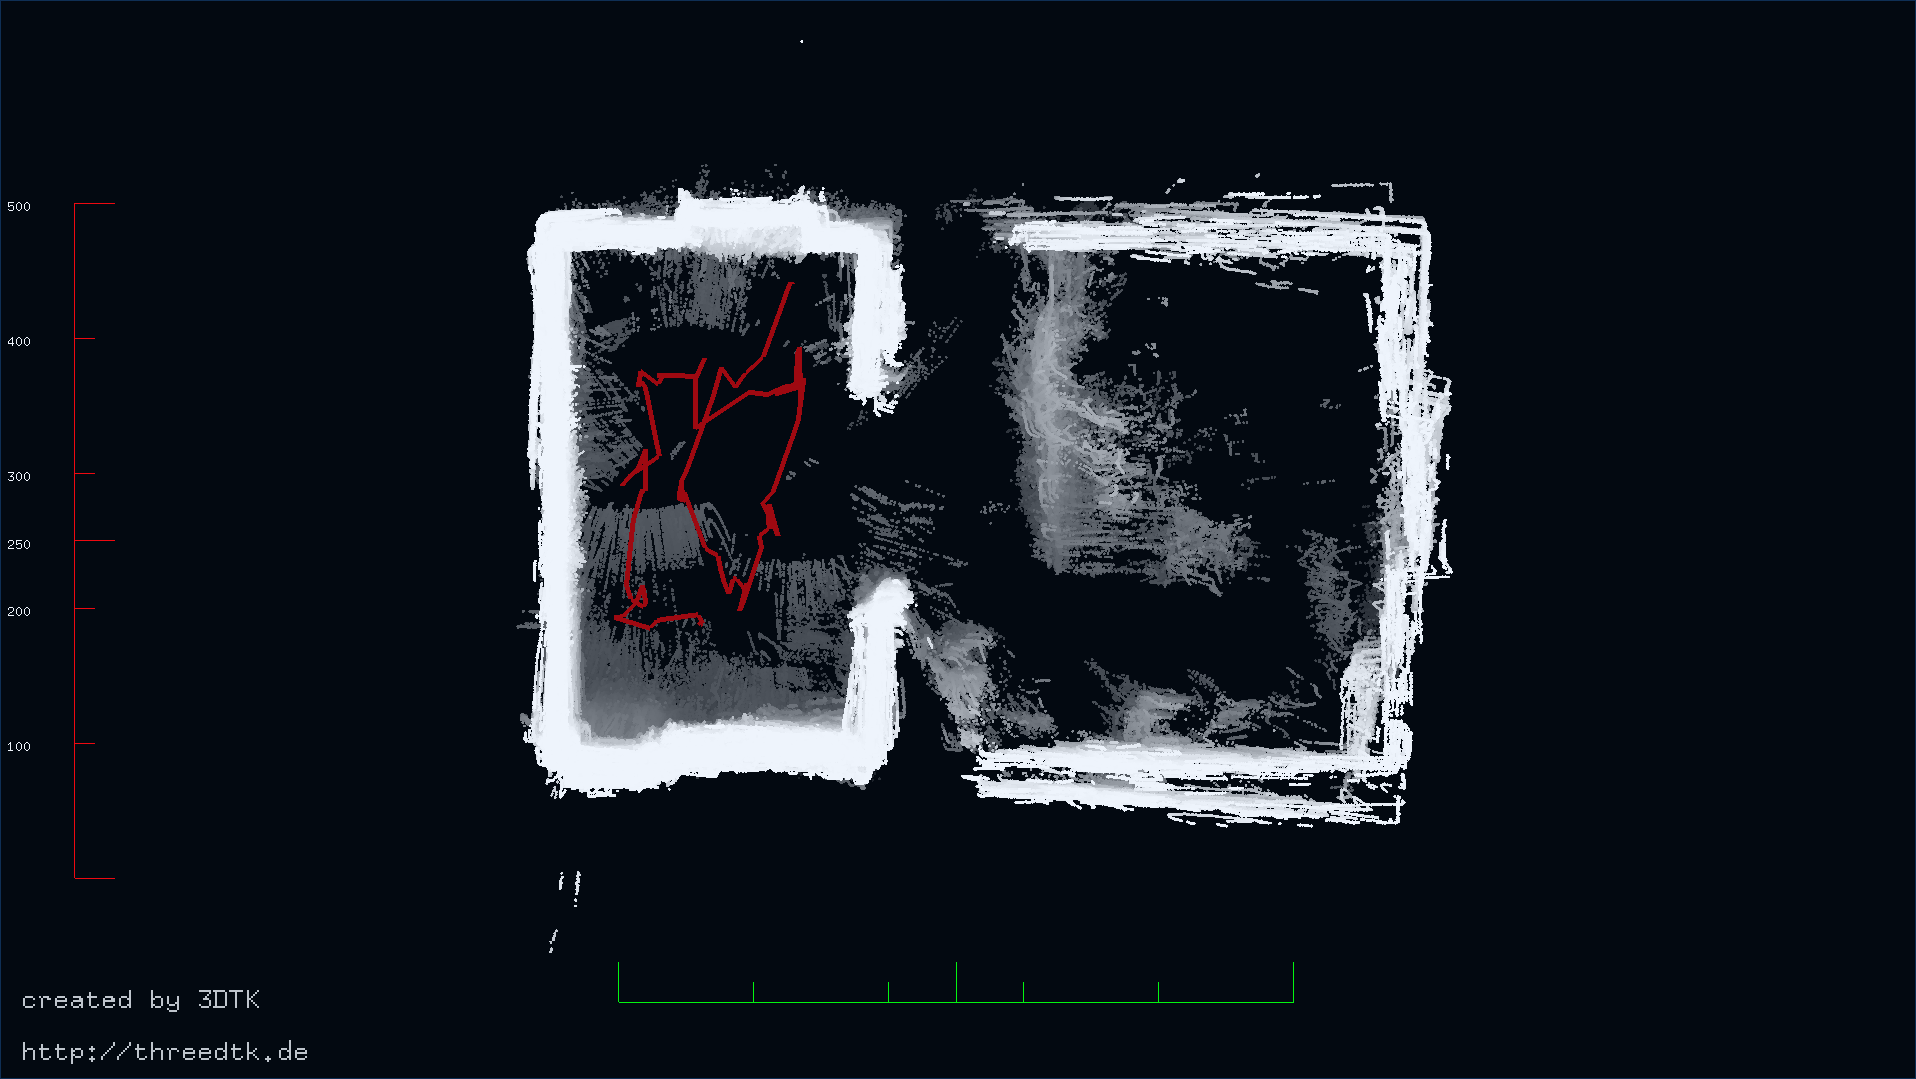
\includegraphics[width=0.495\textwidth]{./images/jasper_corr_top}
        \caption{The point cloud acquired by the rolling sphere before (left) and after (right) applying the plane based registration. View from the interior (top) and a birds-eye view (bottom). Parameters used for optimization: $\epsilon_H = 200$, $\epsilon_P = 300$, $\epsilon_\alpha = \frac{\pi}{4}$, $K = 200$ for AKNN, $d_{growth} = 50$, $N_{c_min} = 800$, $\alpha_0 = [0.001, 0.001, 0.001, 1, 0, 1]^\tau$, $i = 1500$, $k = 1$. An animation of the registration process is given at \url{https://youtu.be/2J8y7MN10JM}.}
        \label{fig:jasperhome}
\end{figure*}
After the registration, the walls of the environment are no longer ambiguous, since all the subsequent scans are matched with the initial plane representation.
When considering the resulting path, it looks distorted.
This is because for some scans, especially empty ones where the sensor points to the ground, no planar features got matched with the global plane model, thus their pose is not optimized.
Improving the path quality is an objective for future works.

% This section is commented out
\iffalse
	\subsection{RADLER Results}

	\subsection{Experimental Results REMOVE THIS SECTION}

	For the experimentally acquired datasets a similar procedure is followed. 
	The main difference being, that the scan was pre-registered using a point-to-point based method as described in section~\ref{sec:experimentalSetup}. 
	Here also the point distances to the ground truth (in this case the terrestrially acquired 3D laser scan) is evaluated before and after the plane-based registration process. 

	\begin{figure}
		\centering
		\begin{minipage}[c]{0.25\textwidth}
			\centering	
			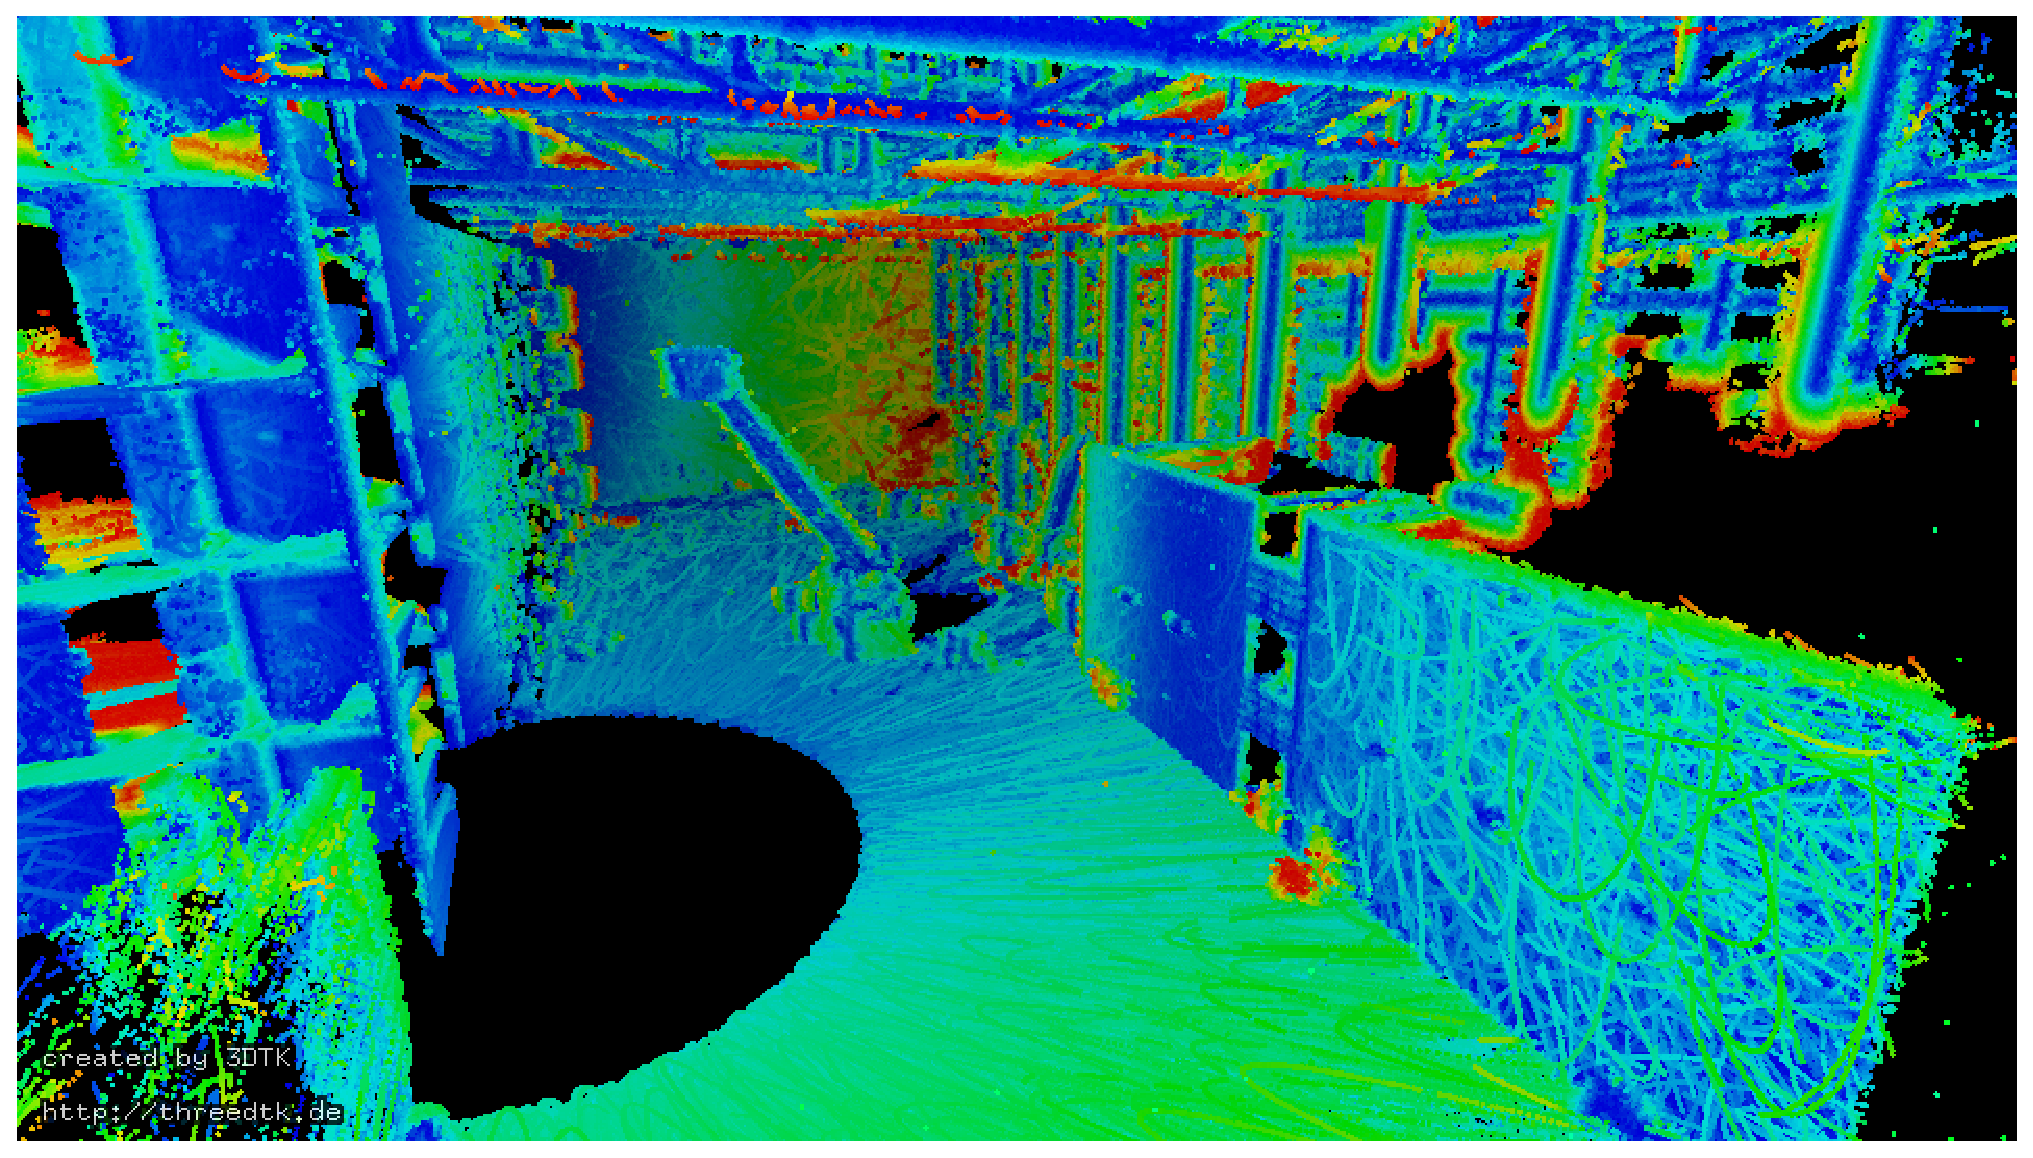
\includegraphics[width = \textwidth]{./images/distances_fire}\\
			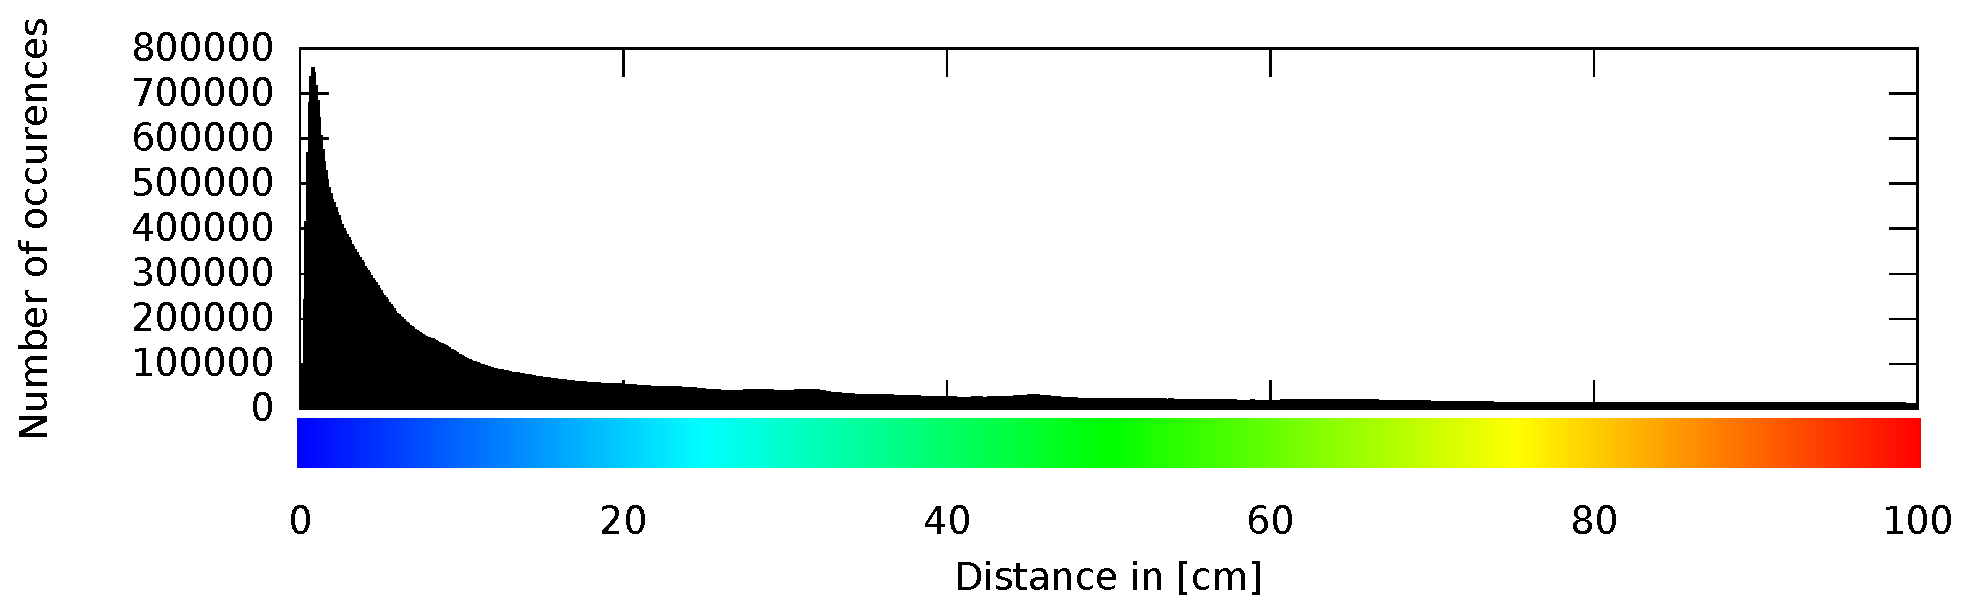
\includegraphics[width = \textwidth]{./images/histogram_fire}
	  	\end{minipage}\hfill
	  	\begin{minipage}[c]{0.25\textwidth}
	  	\end{minipage} 	

		\todo[inline]{Evaluate Plane matching on firefighter school data; histogram after etc}
		\caption{Evaluation of point distances before (left) and after (right) the plane based registration on a experimentally acquired dataset. A maximal distance of \SI{5}{m} is set, such that all points that display a higher distance value are excluded. The left column shows a heat map of distances while the right shows the corresponding histogram. The color mapping is equivalent in both. An animation of the matching process can be seen \href{todo}{here}}
		\label{fig:experimentalEvaluation}
	\end{figure}
\fi
